\subsection{Mixed Reality in der Lehre}
\label{sec-2-2}
\begin{center}
	\fbox{
		\parbox{0.9\linewidth}{
			\textit{Ziel des Kapitels:}\\
			State of the Art in der Überschneidung mit dem Education Bereich vorstellen.\\[6px]
			\textit{Inhalte:}
			\begin{itemize}
				\setlength{\itemsep}{-5pt}
				\item Aktueller Einsatz von MR, insb. der HoloLens, in der Physik
				\item Einsatz von MR in Lehre allgemein, nur relevante Aspekte
			\end{itemize}	
	}}\\	
\end{center}

Ausbildung und Training sind ein wichtiges Anwendungsgebiet für Mixed Reality Technologie. Das gilt besonders für den Bereich der Augmented Realit. In der Literatur findet sich ein breites Spektrum an Arbeiten zum Einsatz von AR zur Vermittlung von Lerninhalten und zum Training. Einige Arbeiten beleuchten die Anwendung von AR aus dem Gesichtspunkt der Lerntheorie, Psychologie und Kognitionsforschung \cite{Marichal17, Santos14}. Andere nähern sich dem Thema aus Sicht konkreter Anwendungsbeispiele und stellen speziell entwickelte AR-Lösungen vor \cite{Strzys17, Amiraslanov18, Buchau09}. Außerdem gibt es eine Reihe von Studien zu den Auswirkungen von AR-Technologie auf das Lernverhalten, den Lernerfolg und die Nutzererfahrung \cite{Ibanez14, Li11, Jerry10, Akcayir16, Strzys18}. Einen Überblick über die Forschung zum Einsatz von AR bei Lernanwendungen geben unter anderem die Arbeiten von Bacca et. al. und Chen et. al. \cite{Chen2017, Bacca14}.\\

Im ersten Schritt beleuchtet das Kapitel kurz allgemeine Erkenntnisse aus der Forschung und stellt dann bestehende Arbeiten zum Einsatz von AR in der Physik vor.

\subsubsection{Einsatz von AR in der Lehre}
In der gängigen Literatur gibt es ein zunehmendes Maß an Arbeiten zur Nutzung von erweiterter Realität in Lernanwendungen \cite{Bacca14, Ibanez18}. Gerade in den Bereichen von Naturwissenschaften und Medizin finden sich hier Beispiele. Oft wurden Anwendungen für Schüler auf Mittel- und Oberstufenniveau sowie angehende Studierende konzipiert. Dabei geht es meist darum, einen Sachverhalt zu erklären und zusätzliche Informationen anzuzeigen. In diesem Zusammenhang werden unter anderem Simulation und Gameification eingesetzt.\\

Die verwendete Hard- und Software variiert dabei. Einige Arbeiten setzen auf Lösungen, die eine Webcam und einen Laptop nutzen. Mit der zunehmenden Verfügbarkeit von Smartphones und Tablets finden sich auch viele Ansätze, die ein solches Gerät nutzen. In der Kategorie der Head Mounted Displays finden sich aufgrund der mangelnden Verfügbarkeit entsprechender Devices vor allem aktuelle Arbeiten auf Basis der HoloLens. Um Darstellung im Raum zu positionieren werden typischerweise Marker-basierte Verfahren genutzt,  aber auch ortsbezogene Informationen wie z.B. eine GPS-Position finden Anwendung.\\

Als positive Auswirkungen von AR-Anwendungen nennen die Arbeiten unter anderem:
\begin{itemize}
	\setlength{\itemsep}{-5pt}
	\item Positiver Lerneffekt
	\item Höheres Motivationslevel und stärkere Interaktivität
	\item Positivere Einstellung und stärkere Einbindung
	\item Verstärkte Kollaboration
\end{itemize}

\begin{comment}
Als Vorteile der Technik werden genannt:
\begin{itemize}
	\item Cognitive Offloading
	\item Intrinsic Contextuality
	\item Spatial and Temporal Contingency
\end{itemize}

\textit{Currently, ARLEs have a mean effect size of 0.56 to student performance with wide variability due to the many possible ways to use AR, as well as, differences in experimental design.} \cite{Santos14}

\vspace{4px}
\textit{Hintergründe aus der Lerntheorie}\\
\textit{Cognitive offloading refers to the possibility of lightening these cognitive demands by the inclusion of actual objects representing abstract concepts. Since these objects are available to the perceptual system they release working memory load} \cite{Marichal17}

\textit{1. Real world annotation improves perception. It juxtaposes real objects, and virtual text and other symbols. This reduces cognitive load in the limited working memory so that a bigger fraction of the STM can be used for operating cognitive processes (e.g., storing in the LTM).
2. Contextual visualization improves elaboration. ARLEs provide more meaningful cues found in the real environment that help a student construct a more elaborate network of knowledge.
3.
Vision-haptic visualization improves elaboration based on embodied imaging. It presents visual information in two modalities: sense of sight and sense of touch.} \cite{Santos14}

\textit{Embodied interactions with science content and new technologies with tangible and gesture-controlled interfaces have started to show enhanced learning effects. This includes environments where the body is cued to enact certain actions and create physical representations that facilitate conceptual understanding. The design rationale is that having learners act out and physicalize the systems, processes, relationships, etc., that they are trying to understand as opposed to externally manipulating these systems and processes (e.g., with a computer mouse) will create conceptual anchors from which new knowledge can be built. Up to this point, there has been little research examining outcomes for students learning the same science content in the same simulation environment, differing only in the degree of immersion and physical interaction with the interface.} \cite{Li11}


\textit{design strategies such as enabling exploration, promoting collaboration, and ensuring immersion to create compelling learning experiences.}\cite{Knierim18}
\end{comment}

%TODO Erst aktuell, dann ältere paper oder andersherum?\\
\subsubsection{In der Physik}
Auch in der Physik finden sich in der gängigen Literatur bereits einige Ansätze, die MR-Technologie nutzen.\\

\vspace{4px}
\textit{holo.lab}\\
Strzys et. al. stellen eine Arbeit vor, in der eine Mixed Reality Anwendung mit der HoloLens im Kontext eines physikalischen Laborversuches genutzt wird \cite{Strzys17}. Dabei handelt es sich um ein Experiment aus der Thermodynamik, bei dem ein Metallstab gleichzeitig von der einen Seite erhitzt und von der anderen gekühlt wird. Nach kurzer Zeit ergibt sich über die Länge des Stabes ein Temperaturverlauf, der mit einer Infrarotkamera gemessen werden kann. Abbildung \ref{img:Strzys17} zeigt den Versuchsaufbau sowie die Szene aus Sicht eines Nutzers mit der HoloLens.\\

\begin{figure}[h!]
	\centering
	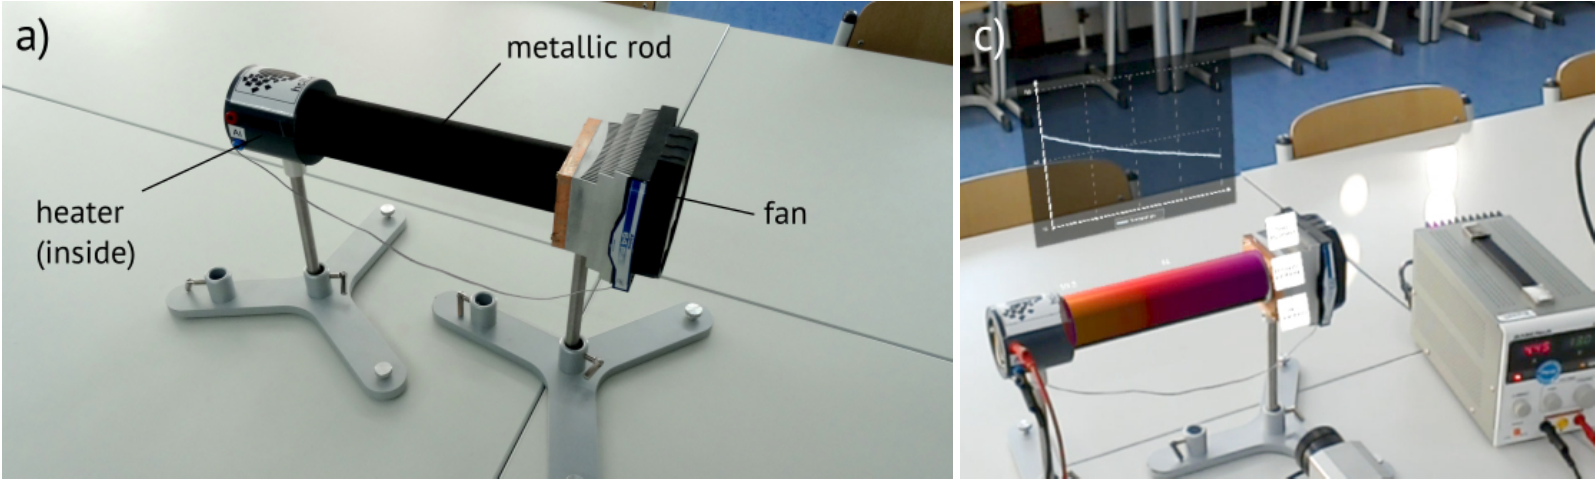
\includegraphics[width=1\textwidth]{images/Strzys18.png}
	\caption{Links: Der zu erhitzende Metallstab. Rechts: Laufendes Experiment aus Sicht eines Nutzers. \cite{Strzys17}}
	\label{img:Strzys17}
\end{figure}

Die Messdaten der Infrarotkamera werden nun in Echtzeit an die HoloLens übertragen, die diese dann auf drei Arten darstellt:
\begin{enumerate}
	\setlength{\itemsep}{-2pt}
	\item Ausgewählte, numerische Werte als Text
	\item Temperaturverlauf als Graph (zweidimensionale Darstellung)
	\item Falschfarbendarstellung über ein eingebettetes 3D-Modell, das den Metallstab überlagert
\end{enumerate}
Dabei hat der Nutzer die Möglichkeit, einzelne Darstellungsformen ein- und auszublenden. Die Autoren schildern den Hintergrund des Designs der Anwendung wie folgt:
\begin{quote}
	\textit{``The main focus of this design is to visualize the invisible and thus to extend human perception to new regimes, e.g., temperature and heat, thereby strengthening the connection between theory and experiment.\\ 
	In this realization the MR setting not only has the advantage of intrinsic contextuality, but also spatial and time contiguity which is supposed to support the learning process of the students. Moreover, the just-in-time evaluation of the data yields the possibility for the students to directly examine the process itself and the parameter involved, and immediately compare the outcome to theoretical predictions which we believe to enhance the links between theory and experiment.''}
\end{quote}
\begin{comment}
%TODO WO ZITIEREN? AN WELCHER STELLE?
\begin{quote}
	\textit{``Under that perspective the effort to achieve possibly more exact numerical values for quantities like the thermal conductivity therefore seem to be less important in this setting. Instead, the technical support during the experimental phase will give students the possibility to thoroughly examine the relationship between cause and effect and thus deepen their physical understanding.''}
\end{quote}
\vspace{4px}
\textit{Demo: Electrical Theories}\\
\end{comment}

\vspace{4px}
\textit{AR in Elektrodynamik}\\
Buchau et. al. stellen eine Arbeit vor, in der ein Verbund aus optischen Markern, Webcam, Laptop und Server genutzt wird, um Magnetfeldlinien für einen Stabmagneten und eine Helmholtz-Spule anzuzeigen. Über die optischen Marker wird die genaue Position und Ausrichtung der Objekte relativ zur Kamera bestimmt. Die Feldlinien werden dann entsprechend in das Bild der WebCam eingebettet und auf dem Laptop angezeigt. Abbildung \ref{img:paper-collection} zeigt zwei Screenshots der Anwendung.\\

\begin{figure}[h!]
	\centering
	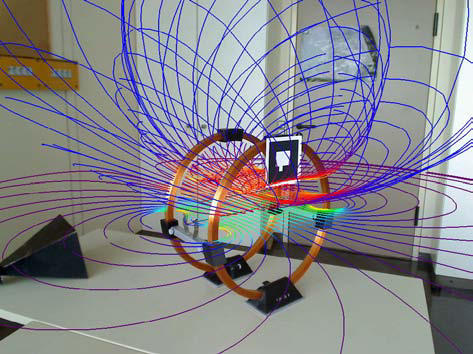
\includegraphics[width=0.45\textwidth]{images/Buchau09.jpg}
	\hspace{0.05cm}
	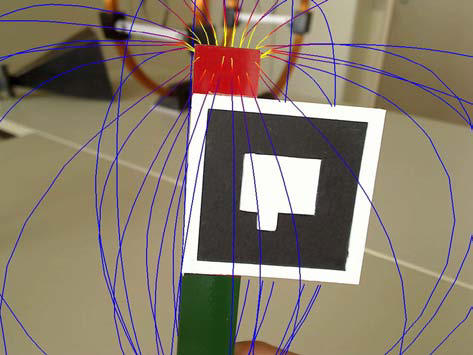
\includegraphics[width=0.45\textwidth]{images/Buchau09_Magnet_2.jpg}
	\caption{\cite{Matsutomo13}}
\end{figure}

Die Berechnung der Feldlinien erfolgt mittels der Finite Elemente Methode auf einem Server. Die Feldstärke ist dabei zusätzlich über die Farbe der Feldlinien codiert. Die Einbettung der errechneten Geometrie in die realen Objekte wird neben der perspektivisch korrekten Darstellung über Verdeckung erzielt. Das geschieht mittels den realen Objekten nachmodellierten, virtuellen Objekten, die anhand der Marker mit den realen Gegenständen überlagert und ausschließlich in den Z-Buffer gerendert werden. Dadurch werden Feldlinien, die sich hinter einem Magneten oder Spulenteil befinden, nicht dargestellt.\\

Die Autoren halten fest, dass Augmented Reality \textit{``eine anschauliche Methode zur Visualisierung elektromagnetischer Felder ist''}. Sowohl Lernende als auch Experten können dabei \textit{``leicht die Charakteristiken der Felder mit den realen Objekten verknüpfen''}. Die vorgestellte Anwendung zielt dabei vor allem auf den Einsatz in einem Unterrichtsraum ab, indem das Bild vom Laptop über einen Beamer für alle Teilnehmer sichtbar gemacht wird.\\

\vspace{4px}
\textit{Weitere Arbeiten}\\
\cite{Amiraslanov18} und \cite{Javaheri18} und \cite{Matsutomo13} und \cite{Mannuss11} und \cite{Jerry10} und \cite{Kaufmann08} und \cite{Techakosit15}

\begin{figure}[h!]
	\centering
	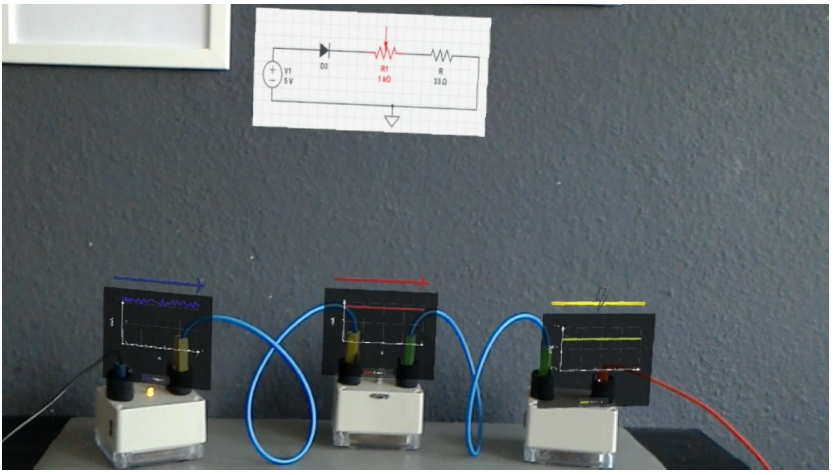
\includegraphics[width=0.45\textwidth]{images/Amiraslanov18.png}
	\hspace{0.05cm}
	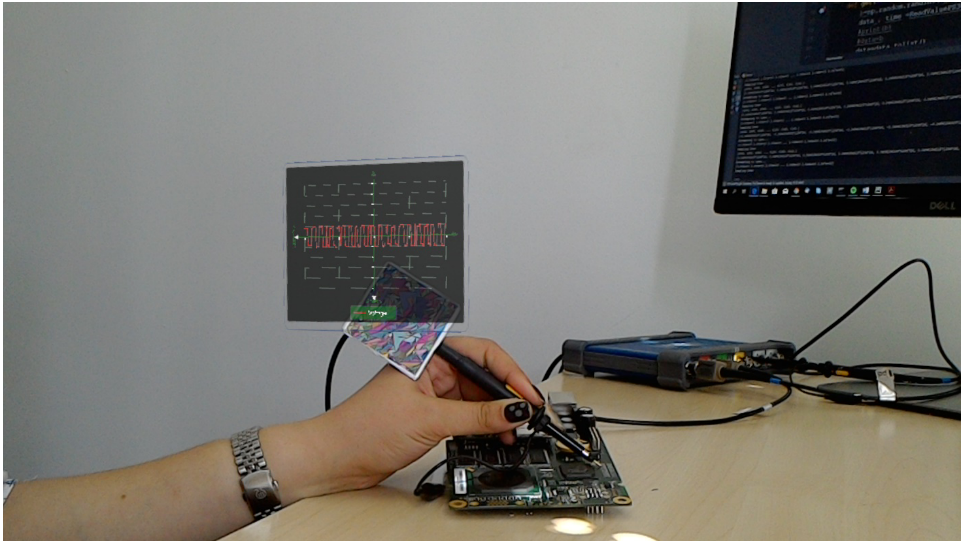
\includegraphics[width=0.45\textwidth]{images/Javaheri18.png}
	\vspace{0.05cm}
	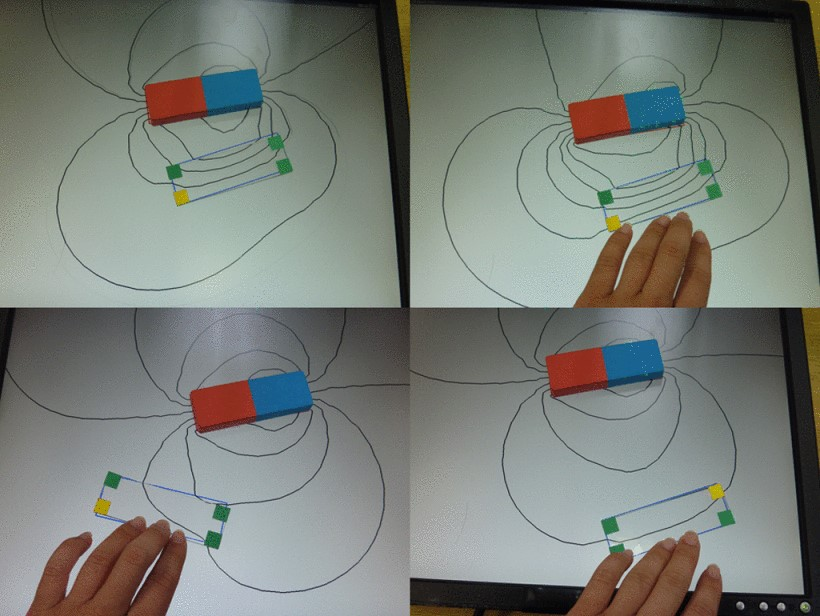
\includegraphics[width=0.45\textwidth]{images/Matsutomo13.jpg}
	\hspace{0.05cm}
	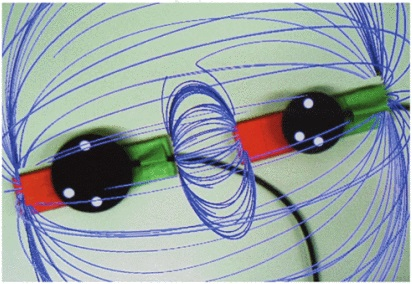
\includegraphics[width=0.45\textwidth]{images/Mannuss11.jpg}
	\caption{\cite{Amiraslanov18} und \cite{Javaheri18} und \cite{Matsutomo13} und \cite{Mannuss11}}
	\label{img:paper-collection}
\end{figure}

\vspace{4px}
\textit{Übersicht über ausgewählte Arbeiten}\\
\setlength\extrarowheight{2pt}
\begin{table}[htb]
	\centering
	\begin{tabular}{l|l|l|l}
		Arbeit & Device & Themengebiet & Fokus\\
		\hline
		\hline
		Strzys et. al. & HoloLens & Thermodynamik & Design \& Studie\\
		\hline
		Amiraslanov et. al & HoloLens & Elektrik & Demo \& Proof of Concept\\
		\hline
		Javaheri et. al. & HoloLens & Elektrik & Demo Anwendung\\
		\hline
		Matsutomo et. al. & WebCam & Magnetismus & Anwendung\\
	\end{tabular}\caption{\label{tab:comparioson} Übersicht}
\end{table}

